\newpage
\section{Lecture-08}
\begin{definition}
A function $f:\mathbb{R}\to\mathbb{R}$ is called \emph{differentiable at $x=a$}
if there exists a real number $L$ such that
\[
\lim_{h\to 0}\frac{f(a+h)-f(a)-Lh}{h}=0.
\]
Then the number $L$ is called the \emph{derivative} of $f$ at $x=a$.
\end{definition}
The definition indicates that,
$$f(a+h)=f(a)+Lh+o(h)$$
So, near $x=a$, the function $f$ behaves like a linear function with slope $L$, $f(a+h) \approx f(a) + Lh=\text{base point}+\text{linear correction}$. The derivative only captures the linear correction part. The constant term just shifts the graph vertically.

\begin{center}
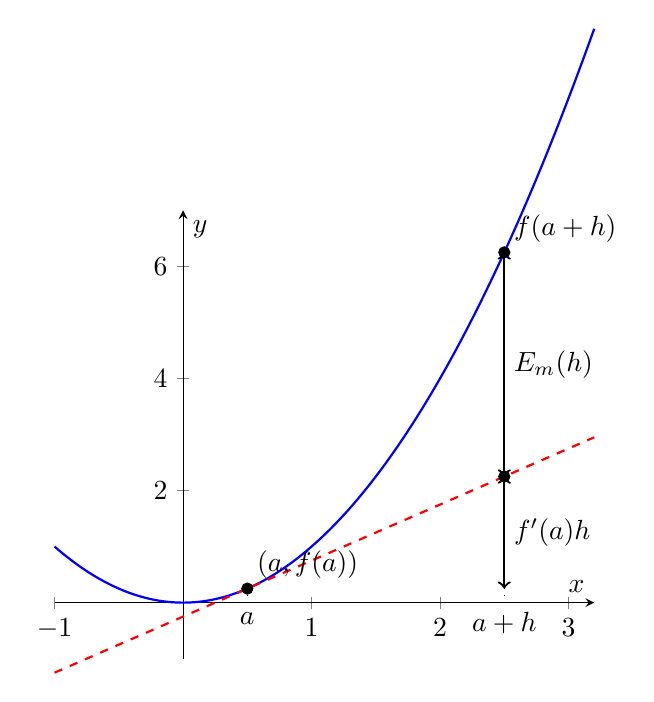
\begin{tikzpicture}
\begin{axis}[
    axis lines = middle,
    xlabel={$x$},
    ylabel={$y$},
    xmin=-1, xmax=3.2,
    ymin=-1, ymax=7,
    samples=200,
    domain=-1:3.2,
    legend style={at={(0.02,0.98)},anchor=north west},
    clip=false
]

% ---- Choose a function (example) ----
% f(x)=x^2, f'(x)=2x
\addplot[blue, thick] {x^2};


% ---- Parameters a and h ----
\def\a{0.5}
\def\h{2}

% Values at a, and at a+h
\pgfmathsetmacro{\fa}{(\a)^2}
\pgfmathsetmacro{\apH}{\a+\h}
\pgfmathsetmacro{\fapH}{(\apH)^2}

% Tangent line at x=a:  y = f(a)+f'(a)(x-a)  ;  f'(a)=2a
\addplot[red, thick, dashed] {2*\a*(x-\a)+\fa};


% Tangent prediction at x=a+h:  L(a+h)=f(a)+f'(a)h
\pgfmathsetmacro{\LapH}{\fa + 2*\a*\h}

% ---- Mark key points ----
\addplot[black, mark=*] coordinates {(\a,\fa)};
\node[above right] at (axis cs:\a,\fa) {$(a,f(a))$};

\addplot[black, mark=*] coordinates {(\apH,\fapH)};
\node[above right] at (axis cs:\apH,\fapH) {$f(a+h)$};

\addplot[black, mark=*] coordinates {(\apH,\LapH)};
% \node[below right] at (axis cs:\apH,\LapH) {$f'(a)h$};

% Vertical reference lines at a and a+h
\addplot[dotted] coordinates {(\a,0) (\a,\fa)};
\node[below] at (axis cs:\a,0) {$a$};

\addplot[dotted] coordinates {(\apH,0) (\apH,\fapH)};
\node[below] at (axis cs:\apH,0) {$a+h$};

% ---- Error: E(h) = f(a+h) - L(a+h) ----
\draw[<->, thick]
  (axis cs:\apH,\LapH) -- (axis cs:\apH,\fapH);

\draw[<->, thick]
  (axis cs:\apH,\fa) -- (axis cs:\apH,\LapH);

\node[right] at (axis cs:\apH, {(\LapH+\fapH)/2})
{$E_m(h)$};
\node[right] at (axis cs:\apH, {(\LapH+\fa)/2})
{$f'(a)h$};
\end{axis}
\end{tikzpicture}
\end{center}

\begin{definition}
A function $f:\mathbb{R}^n \to \mathbb{R}^m$ 
is called \emph{differentiable at $x=\vec a$}
if there exists a linear transformation 
$T_{\vec a}:\mathbb{R}^n \to \mathbb{R}^m$
such that
\[
\lim_{\vec h \to 0}
\frac{
\left\| f(\vec a+\vec h) - f(\vec a) - T_{\vec a}(\vec h) \right\|
}{
\|\vec h\|
}
=0.
\]
Then $T_{\vec a}$ is called the \emph{total derivative} at $x=\vec a$,
and is often denoted by $Df(\vec a)$.
\end{definition}
Again, this says that $Df(\vec a)$ is the best linear approximation to the function $f-f(\vec a)$ at $\vec a$,
in the sense that the difference $f(\vec a+\vec h)-f(\vec a)-Df(\vec a)(\vec h)$ is small compared to $\|\vec h\|$ as $\vec h \to 0$.
\begin{proposition}
    If $f: A \subseteq \R^n \rightarrow \R^m$ is differentiable at $x_0$, then $f$ is continuous at $x_0$.
\end{proposition}
\begin{proof}
    By definition of the derivative of $f$ we know that the limit
$$
\lim_{h \rightarrow 0} \frac{|| f(x_0+h) - f(x_0) + D h || }{||h||} = 0,
$$
for some linear transformation $D$. Therefore since this limit exists, the following is true:
$$
0 = \left( \lim_{h \rightarrow 0} || h ||\right)\left( \lim_{h \rightarrow 0} \frac{|| f(x_0+h) - f(x_0) + D h || }{||h||} \right) = \lim_{h \rightarrow 0} ||f(x_0+h) - f(x_0) + Dh ||.
$$
By the triangle inequality,
$$
\lim_{h \rightarrow 0}||f(x_0+h) - f(x_0) || \leq \lim_{h \rightarrow 0}||f(x_0+h) - f(x_0) +Dh || + \lim_{h \rightarrow 0}||Dh || =\lim_{h \rightarrow 0}||Dh ||.
$$
But since $D$ is linear, it is continuous and $D0=0$, so the lattermost limit is just $0$. Thus $0$ is an upper bound for the limit, but since the norm is always non-negative, this implies that the limit is in fact $0$.
\end{proof}


\begin{proposition}
Suppose there exist two linear transformations
\[
T_{\vec a}^{(1)},\; T_{\vec a}^{(2)} : \mathbb{R}^n \to \mathbb{R}^m
\]
such that
\[
\lim_{\|\vec h\|\to 0}
\frac{
\|f(\vec a+\vec h)-f(\vec a)-T_{\vec a}^{(j)}(\vec h)\|
}{
\|\vec h\|
}
=0,
\qquad j=1,2.
\]
Prove that
\[
T_{\vec a}^{(1)}=T_{\vec a}^{(2)}.
\]
\end{proposition}
\begin{proof}
Since both limits are zero,
\[
T_{\vec a}^{(2)}(\vec h)-T_{\vec a}^{(1)}(\vec h)
=
\{f(\vec a+\vec h)-f(\vec a)-T_{\vec a}^{(1)}(\vec h)\}
-
\{f(\vec a+\vec h)-f(\vec a)-T_{\vec a}^{(2)}(\vec h)\}.
\]
Taking norms and applying the triangle inequality gives
\[
\|(T_{\vec a}^{(2)}-T_{\vec a}^{(1)})(\vec h)\|
\le
\|f(\vec a+\vec h)-f(\vec a)-T_{\vec a}^{(1)}(\vec h)\|
+
\|f(\vec a+\vec h)-f(\vec a)-T_{\vec a}^{(2)}(\vec h)\|.
\]
Dividing by $\|\vec h\|$ and taking the limit yields
\[
\lim_{\|\vec h\|\to 0}
\frac{
\|(T_{\vec a}^{(2)}-T_{\vec a}^{(1)})(\vec h)\|
}{
\|\vec h\|
}
=0.
\]
Let
\[
L := T_{\vec a}^{(2)}-T_{\vec a}^{(1)}.
\]
Then $L$ is linear and
\[
\lim_{\|\vec h\|\to 0}
\frac{\|L(\vec h)\|}{\|\vec h\|}=0.
\]
This only tells us something about vectors $\vec h$ near $\vec 0$.
It does not immediately tell you what $L(\vec h)$ is for a fixed nonzero $\vec h$. Uniqueness needs a statement like the operator is zero on every vector.
The trick plug in $\alpha \vec h$ where $\alpha \to 0$ is exactly how you turn a local limit statement into a global conclusion using linearity.\\
Let $\vec h \neq 0$ be fixed.
For any scalar $\alpha \to 0$, we have $\alpha \vec h \to 0$.
Thus the limit applies:
\[
0=
\lim_{\alpha\to 0}
\frac{
\|L(\alpha \vec h)\|
}{
\|\alpha \vec h\|
}.
\]
By linearity,
\[
L(\alpha \vec h)=\alpha L(\vec h),
\]
so
\[
\frac{
\|L(\alpha \vec h)\|
}{
\|\alpha \vec h\|
}
=
\frac{
\|\alpha L(\vec h)\|
}{
|\alpha|\,\|\vec h\|
}
=
\frac{
\|L(\vec h)\|
}{
\|\vec h\|
}.
\]
\[
0=
\lim_{\alpha\to 0}
\frac{\|L(\alpha \vec h)\|}{\|\alpha \vec h\|}
=
\lim_{\alpha\to 0}
\frac{\|L(\vec h)\|}{\|\vec h\|}.
\]
Notice the quantity inside the limit is constant in $\alpha$.
The limit of a constant sequence/function is just the constant itself. So
\[
\frac{\|L(\vec h)\|}{\|\vec h\|}=0 \implies \|L(\vec h)\|=0.
\]
And the only vector with zero norm is the zero vector. Hence $L(\vec h)=0$.
Since the above holds for every nonzero vector $\vec h$, $L \equiv 0$.
Thus
\[
T_{\vec a}^{(2)}=T_{\vec a}^{(1)}.
\]
\end{proof}